\documentclass[tikz, border=0mm, margin=0mm]{standalone}
\usepackage{tikz}
\usepackage{makecell}%
\usetikzlibrary{shapes.geometric, arrows, positioning, decorations.pathreplacing, calc, matrix, fit}
\usepackage[margin=0.5cm]{geometry}


\begin{document}

% Custom GPU drawing macro
\newcommand{\drawGPU}[3]{
    \begin{scope}[xshift=#1, yshift=#2, scale=#3]
        % GPU Base
        \filldraw[fill=gray!30, draw=black] (0,0) rectangle (7,3);

        % Cooling Fan
        \filldraw[fill=gray!10, draw=black] (1,1.5) circle (0.8);
        \foreach \angle in {0,90,180,270} {
            \draw[thick] (1,1.5) -- ++(\angle:0.8);
        }

        % GPU Components
        \filldraw[fill=gray!50, draw=black] (2.5,2.2) rectangle (4.0,0.8);
        \filldraw[fill=gray!50, draw=black] (5,2.2) rectangle (6.5,0.8);

        % GPU Ports
        \filldraw[fill=black] (-0.2,0.8) rectangle (0,2.2);
    \end{scope}
}

\begin{tikzpicture}[node distance=2cm and 2cm,
  clip,
  inner/.style={draw=black!80,fill=white!20,thick, inner sep=04pt},
  outer/.style={draw=black,fill=white!10,thick,inner sep=06pt},
  mymatrix/.style={matrix of nodes, nodes=typetag, row sep=1em},
  mycontainer/.style={draw=white, inner sep=1ex},
  typetag/.style={draw=white, inner sep=1ex, anchor=west},
  title/.style={draw=none, color=white, inner sep=0pt},
  ]

 \useasboundingbox (-5,-3) rectangle (14,7);

  \node[outer, remember picture,outer xsep=02pt] (input) {
    \begin{tikzpicture}

      \node[] (mapper) {
        \begin{tikzpicture}
          \foreach \y in {0,1,...,8}
            {
            \node[circle, draw=black, fill=green, minimum size=0.01cm, scale=.3] at (0, -\y*0.5) {};
            \node[circle, draw=black, fill=green, minimum size=0.01cm, scale=.3] at (0.1, -\y*0.5) {};
            \node[circle, draw=black, fill=green, minimum size=0.01cm, scale=.3] at (0.2, -\y*0.5) {};
          }
        \end{tikzpicture}
      };

      \node [below=.0cm of mapper] (ssl) {\makecell[c]{Feature vectors \\ (now independent of model)}};

      \matrix[mymatrix, below=0.1cm of ssl, draw] (mx1) {
        |[title]| \\
        % Labels \\
        Annotations \\
      };
      %\node[below=0.0cm of mx1, text width=4.2cm, align=center] (label3) {Annotations};


    \end{tikzpicture}
  };

\coordinate [right=4 of input] (Overfit) {};
  \node[outer, remember picture] (overfit_box) at (Overfit) {
    \begin{tikzpicture}

  \node[inner, remember picture] (finetune) {
    \begin{tikzpicture}
  \node[] (monai) {
    
\includegraphics[width=1.5cm, height=1.5cm]{./MONAI-logo-color.png}
  };

      \node[below=0.0cm of monai]  (pytorch) {
    
\includegraphics[width=1.5cm, height=1.5cm]{./Pytorch_logo.png}
  };
\end{tikzpicture} };
  \node[inner, remember picture, below=0.1cm of finetune] (labelFine) { Linear Probing };

  \node[below=0.0cm of labelFine, text width=4.2cm, align=center] (UMAP) {
    \begin{tikzpicture}
%      \node[] (umap) {
%        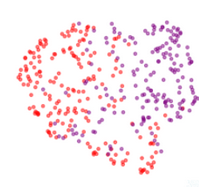
\includegraphics[width=1.5cm, height=1.5cm]{./simpleUmap.png}
%      };
      \node[inner, remember picture] (labelUmap) { UMAP };
    \end{tikzpicture}
    };
    \end{tikzpicture}
 };


 \node[remember picture, below=0.2cm of overfit_box] (omg) {
     \begin{tikzpicture}
         \node[remember picture] (gpuaccel) {
             \begin{tikzpicture}
                 \drawGPU{0}{0}{0.3}
             \end{tikzpicture}
         };
         \node[below=0.00cm of gpuaccel] (labelGPU) { ++ GPU acceleration };

     \end{tikzpicture}
 };

\node[outer, remember picture, right=1.8 of overfit_box] (output) {
    \begin{tikzpicture}

      \node[inner, remember picture] (analysis) { LP scores };

      \node[inner, remember picture, below=0.1cm of analysis] (analysis) { UMAP plots and scores };
    \end{tikzpicture}
  };

\node [above=.0cm of input] (inputText) {Input};
\node [above=.0cm of overfit_box] (overfitText) {Feature inspection plugin};
\node [above=.0cm of output] (outputText) {Output};

\draw[->] (input) -- (overfit_box);
\draw[->] (overfit_box) -- (output);


\end{tikzpicture}

\end{document}

